\newpage
\begin{center}
	\textbf{\large ГЛАВА 4}

	\textbf{\large ВСПОМОГАТЕЛЬНЫЙ МАТЕМАТИЧЕСКИЙ АППАРАТ}
\end{center}
\refstepcounter{chapter}
\addcontentsline{toc}{chapter}{4. ВСПОМОГАТЕЛЬНЫЙ МАТЕМАТИЧЕСКИЙ АППАРАТ}

В рамках данной главы описаны методы, которые применялись для компьютерной реализации теоретических моделей, изложенных в предыдущей главе.

\section{Конечномерная аппроксимация поля в пространстве}
Согласно \ref{generalized_variables}, для моделирования физической системы необходимо уметь задавать некоторые обобщённые переменные в пространсте-времени (пространстве). В данной работе основной формой такого задания являются нейронные сети (по схеме \ref{generalized_variables1}). Однако, для численного поиска минимума \ref{lagrangian_principle1} необходимо много раз производить  интегрирование, и каждое интегрирование требует своего определённого набора точек. В то же время, использование нейронной сети для вычисления в каждой такой точке может быть крайне трудоёмко, поэтому вполне логично, имея нейронную сеть и некоторую белковую молекулу, попробовать построить аппроксимацию поля, создаваемого данной молекулой, и задаваемого нейронной сетью. Использование подобной аппроксимации, хотя и само по себе трудоёмко, может в несколько раз ускорить процесс оптимизации \ref{lagrangian_principle1}. Далее описан подход, позволяющий с определённой долей успеха выполнить такую задачу. 

\subsection{Определение}
Для простоты начнём с одномерного случая. Пусть имеется непрерывная функция $f(x)$, $x \in \mathbb{R}$ такая, что $\exists \intinf f(x) \, dx \in \mathbb{R}$ и
$\lim_{x \to \pm\infty}f(x) = 0$. С помощью сигмоиды, переменной $x \in \mathbb{R}$ можно поставить в соответствие $t \in [0, 1]$:
\begin{equation}
	t = \frac{1}{1 + e^{-x}}.
	\label{t_and_x}
\end{equation}
Обратное преобразование выполняется с помощью функции логит:
\begin{equation}
	x = \ln\frac{t}{1-t}.
	\label{x_and_t}
\end{equation}
Зададим непрерывную функцию $g(t) = f(x) = f(\ln\frac{t}{1-t})$. Из свойств $f$ ясно, что:
\begin{equation}
	g(0) = g(1) = 0,
	\label{g_zeros}
\end{equation}
а также, что $\int_0^1g(t) \, dt \in \mathbb{R}$.

Из-за \ref{g_zeros} функция $g$ может быть продолжена как нечётная на $[-1, 1]$, а следовательно -- быть разложена в ряд Фурье по синусам:
\begin{equation}
	g(t) = \sum_{i=1}^\infty a_i\sin{\pi it},
	\label{fourier}
\end{equation}
где:
\begin{equation}
	a_i = 2\int_0^1g(t) \sin{\pi it} \, dt.
	\label{a_coef}
\end{equation}

Ряд \ref{fourier} сходится равномерно. Через него можно записать функцию $f(x)$:
\begin{equation}
	f(x) = \sum_{i=1}^\infty a_i\sin{\frac{\pi i}{1 + e^{-x}}},
	\label{logit_fourier}
\end{equation}
а коэффициент $a_i$ перепишется как:
\begin{equation}
	a_i = 2\int_0^1f(\ln\frac{t}{1-t}) \sin{\pi it} \, dt = 2\intinf f(x)\sin(\frac{\pi i}{1+e^{-x}})\frac{e^{-x}}{(1+e^{-x})^2}\, dx.
	\label{a_coef_logit}
\end{equation}
Раз \ref{fourier} сходится равномерно, то и \ref{logit_fourier} сходится равномерно.

Далее будет необходимо воспользоваться двумя известными функциями:
\begin{itemize}
\item $\si(x) = \int_0^x\frac{\sin t}{t}\, dt$ -- интегральный синус;
\item $\cin(x) = \int_0^x\frac{1 - \cos t}{t}\, dt$ -- интегральный косинус.
\end{itemize}

Если в \ref{fourier} имеем дело с разложением функции $g(t)$ по ортонормированному базису из функций $2\sin{\pi it}$, то в случае с \ref{logit_fourier}
последовательность функций $\sin{\frac{\pi i}{1 + e^{-x}}}$ не явлется ни нормированной, ни попарно ортогональной. Рассчитаем основные интегралы, связанные с \ref{logit_fourier}:
\begin{align}
	&\intinf\sin{\frac{\pi i}{1+e^{-x}}} \, dx = \int_0^1\sin{\pi it} \, d\ln{\frac{t}{1-t}} = \int_0^1 \frac{\sin{\pi it}}{t(1-t)} \, dt = \notag \\
	&= \int_0^1 \frac{\sin{\pi it}}{t} \, dt + \int_0^1 \frac{\sin{\pi it}}{1-t} \, dt = \int_0^1 \frac{\sin{\pi it}}{t} \, dt - \int_0^1 \frac{\sin{(\pi - \pi i\xi)}}{\xi} \, d\xi = \notag \\
	&= \int_0^1 \frac{\sin{\pi it}}{t} \, dt - {(-1)}^i\int_0^1 \frac{\sin{\pi i\xi}}{\xi} \, d\xi = (1 + {(-1)}^{i+1})\si(\pi i).
	\label{f_int}
\end{align}
Формула \ref{f_int} позволяет при наличии коэффициентов \ref{a_coef} посчитать интеграл функции $f(x)$ по всей числовой прямой. Пусть имеются две функции $f^1(x)$ и $f^2(x)$, которые разлагаются по \ref{logit_fourier} с коэффициентами $a^1_i$ и $a^2_j$. Крайне полезно уметь считать интеграл $\intinf f^1(x)f^2(x)\, dx$ (сравните с \ref{action_function_two} и \ref{L_partial_multiscalar}), что было бы крайне легко, если бы последовательность функций $\sin{\frac{\pi i}{1 + e^{-x}}}$ была ортонормированной, но так как это не так, необходимо рассчитать интегралы попарных произведений функций этой последовательности:

\begin{align}
	&\intinf\sin{\frac{\pi i}{1+e^{-x}}}\sin{\frac{\pi j}{1+e^{-x}}} \, dx = \int_0^1\sin{\pi it}\sin{\pi jt} \, d\ln{\frac{t}{1-t}} = \notag \\
	&= \int_0^1\frac{\cos\pi (i-j)t - \cos\pi (i+j)t}{2}\left(\frac{1}{t} + \frac{1}{1-t}\right)\, dt = \frac{1}{2}(\int_0^1\frac{1-\cos\pi (i+j)t}{t}\, dt - \notag \\
	&- \int_0^1\frac{1-\cos\pi (i-j)t}{t}\, dt + \int_0^1\frac{\cos\pi (i-j)t-\cos\pi (i+j)t}{1-t}\, dt) = \frac{1}{2}(\cin(\pi(i+j)) -\notag \\
	&- \cin(\pi(i-j)) + \int_0^1\frac{{(-1)^{i-j}}\cos\pi(i-j)\xi - {(-1)^{i+j}}\cos\pi(i+j)\xi}{\xi}\, d\xi) = \notag \\
	&= \frac{1+{(-1)}^{i+j}}{2}\left(\cin(\pi(i+j)) - \cin(\pi(i-j))\right).
	\label{fg_int}
\end{align}

Из \ref{fg_int} при $i=j$ получим:
\begin{equation}
	\intinf\sin^2\frac{\pi i}{1+e^{-x}}\, dx = \cin(2\pi i).
	\label{f_sqr_int}
\end{equation}

Так как в рамках исследуемой задачи необходимо аппроксимировать функции заданные на трёхмерном, а не одномерном пространстве, то следует перейти к трёхмерному ряду Фурье.
Для такого ряда формулу \ref{logit_fourier} перепишем как:
\begin{equation}
	f(x,y,z) = \sum_{i,j,k=1}^\infty A_{i,j,k}\sin{\frac{\pi i}{1 + e^{-x}}}\sin{\frac{\pi j}{1 + e^{-y}}}\sin{\frac{\pi k}{1 + e^{-z}}},
	\label{logit_fourier_3d}
\end{equation}
где:
\begin{equation}
	A_{i,j,k} = 2^3\iiint_{\mathbb{R}^3}\frac{f(x, y, z)\sin\frac{\pi i}{(1+e^{-x})^2}\sin\frac{\pi j}{(1+e^{-y})^2}\sin\frac{\pi k}{(1+e^{-z})^2}e^{-x-y-z}}{(1+e^{-x})^2(1+e^{-y})^2(1+e^{-z})^2}\, d^3x.
	\label{a_coef_logit_3d}
\end{equation}

Легко видеть, что формулы \ref{f_int}, \ref{fg_int} и \ref{f_sqr_int} полезны и для трёхмерного случая.

\subsection{Вычисление коэффициентов по методу Монте-Карло}

При построении аппроксимации, во-первых, приходится ограничиваться некоторым конечным числом слагаемых ряда, а во-вторых, необходимо численно получать значения коэффициентов \ref{a_coef_logit_3d}. Из-за относительно большой размерности функции, и необходимости считать интегралы по всему пространству, интегрирование по сетке точек не так удобно -- проще применить метод Монте-Карло.

Для метода Монте-Карло необходимо иметь некоторую трёхмерную случайную величину $\xi = {[\xi_x, \xi_y, \xi_z]}^\mathrm{T}$, принимающую все значения из $\mathbb{R}^3$ с распределением вероятности $p(x, y, z)$ ($p > 0$, $\iiint_{\mathbb{R}^3}p(x, y, z)\, dx\, dy\, dz = 1$). На роль такой случайной величины хорошо подходит многомерное нормальное распределение. Хорошо известно, что для любой функции $f(x, y, z)$ можно записать:
\begin{equation}
	\iiint_{\mathbb{R}^3}f(x,y,z)\, dx\, dy\, dz=\iiint_{\mathbb{R}^3}\frac{f(x,y,z)}{p(x,y,z)}p(x,y,z)\, dx\, dy\, dz=\E{\frac{f(\xi)}{p(\xi)}},
	\label{monte-carlo1}
\end{equation}
из чего, при наличии $N$ выборочных значений $\xi^i$, через статистическую оценку среднего получаем:
\begin{equation}
	\iiint_{\mathbb{R}^3}f(x,y,z)\, dx\, dy\, dz=\E{\frac{f(\xi)}{p(\xi)}} \approx \frac{1}{N}\sum_{i=1}^N\frac{f(\xi^i)}{p(\xi^i)}.
	\label{monte-carlo2}
\end{equation}
Использование формулы \ref{monte-carlo2} совместно с \ref{a_coef_logit_3d} даёт искомую аппроксимацию.

Достоинством описанного выше метода является, как минимум, то, что он работает, и позволяет с некоторой точностью записать многомерную, заданную на всём бесконечном множестве функцию, используя конечное число параметров. Следует также привести недостатки данного метода:
\begin{enumerate}
\item При ограниченном числе членов ряда, точность приближения крайне чувствительна к сдвигам приближаемой функции ($f(x, y, z) \to f(x+c_x, y+c_y, z+c_z)$). Это выражается в том плане, что  не следует сразу использовать \ref{a_coef_logit_3d}, вместо этого следует искать такое преобразование исходных координат -- желательно линейное $x = A\hat{x} + b$, для которого отклонение аппроксимации $\hat{f}$ от исходной $f$ будет минимальным:
\begin{align}
	&A'_{i,j,k} = 2^3\iiint_{\mathbb{R}^3}\frac{f(Ax+b)\sin\frac{\pi i}{(1+e^{-(a_{11}x+a_{12}y+a_{13}z+b_1)})^2}\cdot...\cdot e^{-((a_{11}+...)x+...)}}{(1+e^{-(a_{11}x+a_{12}y+a_{13}z+b_1)})^2\cdot...}\, d^3x,
	\label{a_coef_logit_3d_mod}
\end{align}
\begin{equation}
	\hat{f}(x,y,z) = \det(A)\sum_{i,j,k=1}^\infty A'_{i,j,k}\sin{\frac{\pi i}{1 + e^{-(a_{11}x+a_{12}y+a_{13}z+b_1)}}}\cdot...,
	\label{logit_fourier_3d_mod}
\end{equation}
и
\begin{equation}
	\iiint_{\mathbb{R}^3}{(f(x) - \hat{f}(x))}^2\,d^3x \to \min.
	\label{a_coef_logit_3d_mod_cond}
\end{equation}
Поиск \ref{a_coef_logit_3d_mod_cond} эффективно выполняется с помощью методов градиентного спуска.

\item Точность приближения также сильно зависит от дисперсии распределения $\xi$. Если дисперсия слишком мала, она может не покрыть всех особенностей функции $f$.

\item Увеличение количества учитываемых членов ряда Фурье приводит к увеличению точности, но в многомерном случае приводит к очень быстрому росту трудоёмкости вычислений, а формулы \ref{f_int}, \ref{fg_int} и \ref{f_sqr_int} становятся малоприменимыми.

\item Метод Монте-Карло обладает высокой дисперсией, его точность растёт со скоростью $O(\frac{1}{\sqrt{N}})$. Вместе с разложением в ряд Фурье и недостаточно большими значениями $N$ приводят к быстрому накоплению ошибок.
\end{enumerate}

\subsection{Графические примеры}
Приведём несколько графических примеров описанного выше подхода для аппроксимации одномерных функций и двумерных изображений.
\begin{figure}[H]
	\centering
	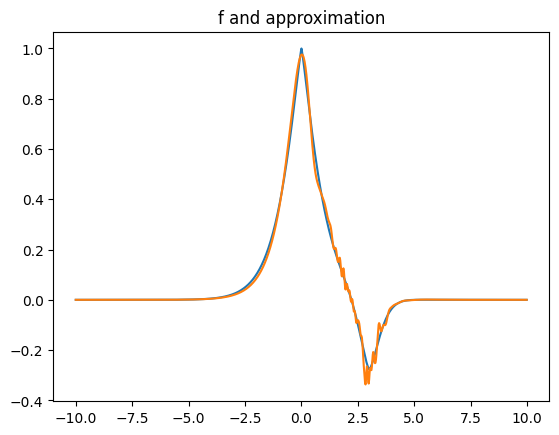
\includegraphics[scale=0.9]{plot1.png}
	\caption{Приближение функции $f(x) = e^{-|x|^{1,2}} - 0,3e^{-2|x-3|^{1,5}}$.}
	\label{fig_plot1}
\end{figure}
\begin{figure}[H]
	\centering
	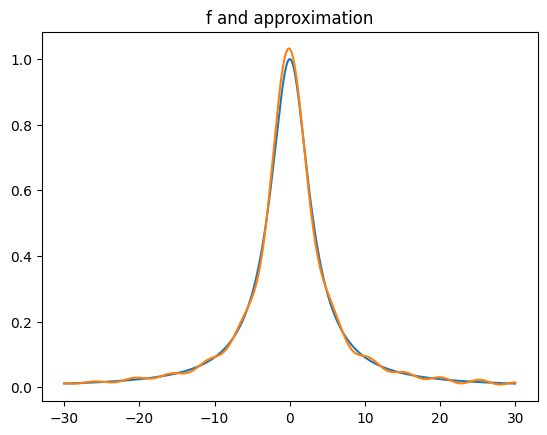
\includegraphics[scale=0.9]{plot2.png}
	\caption{Приближение функции $f(x) = \frac{10}{10 + x^2}$.}
	\label{fig_plot2}
\end{figure}
\begin{figure}[H]
	\centering
	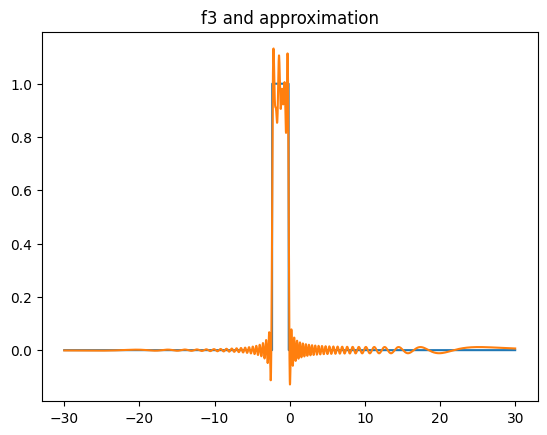
\includegraphics[scale=0.9]{plot3.png}
	\caption{Приближение функции $f(x) = \mathbb{I}[|x + 1,25| < 1,1]$.}
	\label{fig_plot3}
\end{figure}
\begin{figure}[H]
	\centering
	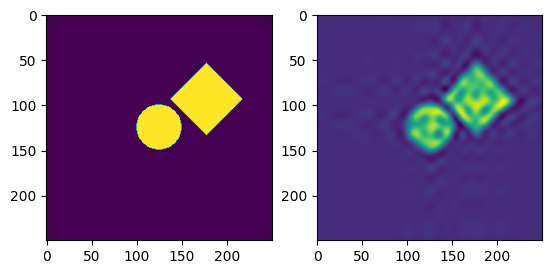
\includegraphics[scale=0.8]{imag1.png}
	\caption{Приближение круга и квадрата.}
	\label{fig_imag1}
\end{figure}
\begin{figure}[H]
	\centering
	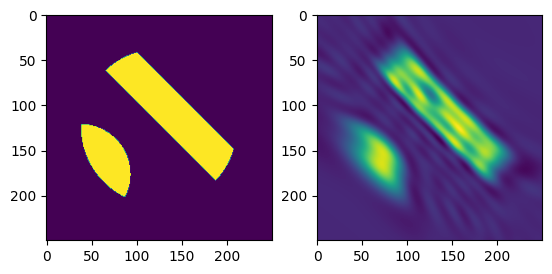
\includegraphics[scale=0.8]{imag2.png}
	\caption{Приближение пересечения круга с объединением круга и прямоугольника.}
	\label{fig_imag2}
\end{figure}
\begin{figure}[H]
	\centering
	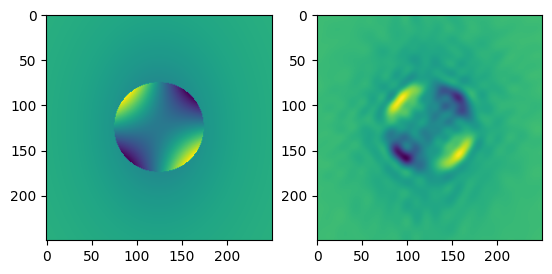
\includegraphics[scale=0.8]{imag3.png}
	\caption{Приближение функции $f(x, y) = \frac{xy}{10}\mathbb{I}[|x^2 + y^2| < 4] - \frac{1}{10 + x^2 + y^2}$.}
	\label{fig_imag3}
\end{figure}

\section{Параметризация пары взаимодействующих молекул}
Взаимодействие двух белковых молекул проще всего моделировать как взаимодействие двух жёстких тел. В общем случае, все конформации получаемого комплекса можно записать с помощью 6 параметров: одна компонента фиксируется, для второй компоненты выбирается центр (3 параметра) и поворот (3 параметра). В случае, когда компоненты идентичны (гомодимерные комплексы), в силу определённой симметрии, можно обойтись всего 4 параметрами.

Воспользовавшись физическими соображениями, можно попробовать сократить необходимое число параметров на 1. Для этого можно воспользоваться \textit{операцией <<сталкивания>>}\cite{prip2023}. Она заключается в том, чтобы найти такое минимальное расстояние между молекулами, при котором минимальное расстояние между C\textalpha-атомами не превышает некоторой границы (обычно ван-дер-ваальсовых радиусов атомов углерода -- 3,4\AA{}, но можно, например, 3,6\AA{}). Ранее, такая операция выполнялась с помощью итеративного процесса, при котором молекулы раздвигаются с некоторым постоянным шагом, пока условие о ненарушении границ не будет выполнено. В рамках же данной работы операция выполняется с помощью метода дихотомии.

При использовании моделей типа \ref{action_function}, необходимо выполнение интегрирования по всему пространству, что может быть выполнено с помощью метода Монте-Карло \ref{monte-carlo2}. Поиск решения \ref{lagrangian_principle_practical} заключается в итеративном интегрировании \ref{monte-carlo2}, изменении параметров комплекса, дальнейшем интегрировании, изменении параметров и т.д. Если при каждом интегрировании \ref{monte-carlo2} случайная выборка $\xi^i$, $i=\overline{1,N}$ генерируется заново, то возникает дополнительная дисперсия, которая мешает процессу оптимизации. Чтобы избежать этой проблемы, можно сгенерировать единое случайное облако $\xi^i$, $i=\overline{1,N}$ и применять его на всех итерациях. Впрочем, возникает проблема такого рода, что такое фиксированное облако может оказаться слишком маленьким и не покрывать всех возможных конформаций комплекса.

Чтобы как-то обойти данную проблему, можно использовать другую параметризацию. В ней центры молекул задаются через параметр $r$ как: $[-r, 0, 0]^\mathrm{T}$ и $[r, 0, 0]^\mathrm{T}$. Поворот каждой из молекул задаётся 3 параметрами, что приводит к тому, что итоговое количество параметров равно 7 (если использовать операцию сталкивания для поиска параметра $r$ при заданных поворотах, то можно сократить количество параметров до 6). Тогда случайную величину $\xi$ можно генерировать из многомерного нормального распределения, достаточно протяжённого относительно оси $[1, 0, 0]^\mathrm{T}$.

\section{Алгоритмы оптимизации}
В рамках данного исследования были использованы различные методы оптимизации. При обучении нейронный сетей, а также при решении \ref{a_coef_logit_3d_mod_cond}, используется популярный алгорит стохастической оптимизации Adam\cite{adam}. Впрочем, при решении \ref{lagrangian_principle_practical} данный алгоритм оказался малоприменим. Во-первых, при моделировании часто использовались плохо дифференцируемые функции. Во-вторых, из-за наличия малой относительно малого (по сравнению с нейронными сетями) количества параметров, алгоритм не способен достичь глобального минимума. Для решения данных проблем, предлагается использовать эволюционные методы оптимизации \cite{evol_methods}.

\subsection{Простой эволюционный алгоритм}
Был использован простой эволюционный алгоритм следующего вида. Пусть $p$ -- вектор параметров (кодирует форму взаимодействие), $f(p)$ -- минимизируемая функция (частичный лагранжиан),
$g(p)$ -- бинарная функция, сигнализирующая некорректные параметры (функция, сигнализирующая нарушение радиусов ван-дер-ваальса):
\begin{algorithm}
\begin{algorithmic}
\State $P \gets [p_1, p_2, ..., p_N]$ из многомерного равномерного распределения с заданными границами;
\State $p_{best} \gets null$;
\State $f_{best} \gets +\infty$;
\State $iter \gets 0$;
\While{$iter < I$}
	\State $P_{rand} \gets [p_1, p_2, ..., p_{N_{rand}}]$ из многомерного равномерного распределения с заданными границами;
	\State $P_{mut} \gets P + [\delta{}p_1, \delta{}p_2, ..., \delta{}p_{N_{mut}}]$, где $\delta{}p_i$ из многомерного нормального распределения с заданной дисперсией;
	\State $P_{parent_1} \gets [p_{i_1}, p_{i_2}, ..., p_{i_{N_{parent}}}]$, где $i_j$ -- случайная выборка из популяции;
	\State $P_{parent_2} \gets [p_{j_1}, p_{j_2}, ..., p_{j_{N_{parent}}}]$ (аналогично);
	\State $P_{cross} \gets \alpha P_{parent_1} + (1 - \alpha)P_{parent_2}$, где $\alpha = [\alpha_1, ..., \alpha_{N_{parent}}]$ из $\mathbb{U}[0, 1]$;
	\State $P \gets [P | P_{rand} | P_{mut} | P_{cross}]$;
	\State $P \gets \{p | \forall p \in P: g(p) = 0\}$;
	\State $F \gets [f(p_1), f(p_2), ...]$;
	\State Пусть $F_{sorted}$, $P_{sorted}$ отсортированые массивы (по возрастанию $F$);
	\State $f_{iterbest} \gets (F_{sorted})_1$, $p_{iterbest} \gets (P_{sorted})_1$;
	\If{$f_{iterbest} < f_{best}$}
		\State $p_{best} \gets p_{iterbest}$;
		\State $f_{best} \gets f_{iterbest}$;
	\EndIf
	\If{$\len(P_{sorted}) < N$}
		\State $P_{sorted} \gets [P_{sorted} | p_{\len(P_{sorted})+1}, ..., p_N]$ (добавление случайных параметров); 
	\EndIf
	\State $P \gets [(P_{sorted})_1, (P_{sorted})_2, ..., (P_{sorted})_N]$;
	\State $iter \gets iter+1$;
\EndWhile
\State Результат: $(p_{best}, f_{best})$.
\end{algorithmic}
\end{algorithm}

\subsection{Роевая оптимизация}
Другим использованным эволюционным алгоритмом является роевая оптимизация. В данной работе использовалась простая версия такого алгоритма, в ней все итерации, следующие за исходной генерацией параметров являются детерминированными. Используя те же обозначения, что и для предыдущего алгоритма, но не используя $g(p)$, запишем:
\begin{algorithm}
\begin{algorithmic}
\State $P \gets [p_1, p_2, ..., p_N]$ из многомерного равномерного распределения с заданными границами;
\State $V \gets [\vec{0}, \vec{0}, ..., \vec{0}]$;
\State $P_{itembest} \gets [null, ..., null]$;
\State $F_{itembest} \gets [+\infty, ..., +\infty]$;
\State $p_{best} \gets null$;
\State $f_{best} \gets +\infty$;
\State $iter \gets 0$;
\While{$iter < I$}
	\State $F = [f(p_1), f(p_2), ..., f(p_N)]$;
	\State Для $i=\overline{1,N}$, если $F_i < (F_{itembest})_i$: $(F_{itembest})_i \gets F_i$;
	\State Для $i=\overline{1,N}$, если $F_i < (F_{itembest})_i$: $(P_{itembest})_i \gets P_i$;
	\State $f_{iterbest} \gets \min{F_i}$;
	\State $p_{iterbest} \gets \min{P_i}$;
	\If{$f_{iterbest} < f_{best}$}
		\State $p_{best} \gets p_{iterbest}$;
		\State $f_{best} \gets f_{iterbest}$;
	\EndIf
	\State $V \gets \beta(\alpha_{loc}(P_{itembest} - P)+\alpha_{glob}(p_{best} - P)) + (1-\beta)V$;
	\State $P \gets P + V$;
	\State $iter \gets iter+1$;
\EndWhile
\State Результат: $(p_{best}, f_{best})$.
\end{algorithmic}
\end{algorithm}